\section{The Phong Illumination Model}

\begin{frame}{Phong Model: History}
  \begin{columns}
    \begin{column}{0.7\textwidth}
      \small
      \begin{conceptbox}{Historical Context}
        Developed by \textbf{Bui Tuong Phong} as his PhD dissertation at the University of Utah in 1973.

        \textbf{Goal:} Fast, realistic-looking lighting
      \end{conceptbox}
      In Phong's words:

      \begin{quote}
        \footnotesize
        "We do not expect to be able to display the object exactly as it would appear in reality, with texture, overcast shadows, etc. We hope only to display an image that approximates the real object closely enough to provide a certain degree of realism."
      \end{quote}
      {\small
        Phong completed his PhD in only \textbf{two years}, a record at the time. Yet tragically, he died of cancer only two years later.
      }
    \end{column}
    \begin{column}{0.3\textwidth}
      \begin{figure}
        \centering
        \includegraphics[width=\linewidth]{images/phong.jpg}
        \caption*{Bui Tuong Phong (1942-1975)}
      \end{figure}
    \end{column}
  \end{columns}
\end{frame}

\begin{frame}{Phong Model Overview}
  \begin{columns}
    \begin{column}{0.6\textwidth}
      \begin{mathbox}{Phong Formula}
        \small
        Break lighting into three components that can be computed independently
        \begin{align*}
          I &= I_{\text{ambient}} + I_{\text{diffuse}} + I_{\text{specular}} \\
          &= k_a I_a + k_d \mathbf{I}_l (\mathbf{N} \cdot \mathbf{L}) + k_s \mathbf{I}_l (\mathbf{R} \cdot \mathbf{V})^n
        \end{align*}
      \end{mathbox}
    \end{column}
    \begin{column}{0.4\textwidth}
      \begin{tikzpicture}[scale=0.8]
        % Surface
        \draw[ObjectColor, very thick] (-2,0) -- (2,0);
        \fill[ObjectColor] (0,0) circle (3pt);

        \node[eye] (eye) at (3, 1.5) {\faIcon{eye}};
        \node[circle, fill=LightColor, minimum size=0.5cm] (light) at (-2,2) {\footnotesize \faIcon{lightbulb}};

        \draw[->, PrimaryColor, thick] (0,0) -- (0,1.5) node[above, anchor=south] {\footnotesize $\mathbf{N}$};

        \draw[->, lightray, thick] (0,0) -- (-1.2,1.2) node[above, anchor=south] {\footnotesize $\mathbf{L}$};

        \draw[->, AccentColor, thick] (0,0) -- ($0.5*(eye)$) node[above, anchor=south] {\footnotesize $\mathbf{V}$};

        % Reflection vector
        \draw[->, reflectray, thick] (0,0) -- (1.2,1.2);
        \node[above right] at (1,1.4) {\footnotesize $\mathbf{R}$};

      \end{tikzpicture}
    \end{column}
  \end{columns}

  \vspace{0.3cm}
  \only<2>{
    \begin{figure}
      \centering
      \includegraphics[width=0.9\linewidth]{images/phong_components.png}
      \caption*{Phong model components}
    \end{figure}
  }
\end{frame}

\begin{frame}{Types of Reflection}
  \begin{columns}
    \begin{column}{0.4\textwidth}
      \begin{tikzpicture}[scale=0.8]
        \draw[ObjectColor, very thick] (-2,2) -- (2,2);
        \node[above] at (0,3.5) {\scriptsize Smooth Surface};

        \draw[lightray] (-1.5,3.5) -- (-0.5,2);
        \draw[lightray] (-0.5,3.5) -- (0.5,2);
        \draw[lightray] (0.5,3.5) -- (1.5,2);

        \draw[reflectray] (-0.5,2) -- (-1.5,0.5);
        \draw[reflectray] (0.5,2) -- (-0.5,0.5);
        \draw[reflectray] (1.5,2) -- (0.5,0.5);

        \node[below] at (0,0.6) {\scriptsize Specular Reflection};
        \node[below] at (0,0.4) {\scriptsize (Mirror-like)};

        \only<2->{
          \begin{scope}[shift={(0, -2)}]
            \draw[ObjectColor, very thick, decoration={snake, amplitude=1pt}, decorate] (-2,-0.5) -- (2,-0.5);
            \node[above] at (0,1) {\scriptsize Rough Surface};

            \draw[lightray] (-1.5,1) -- (-0.5,-0.5);
            \draw[lightray] (-0.5,1) -- (0.5,-0.5);
            \draw[lightray] (0.5,1) -- (1.5,-0.5);

            \draw[reflectray] (-0.5,-0.5) -- (-1.2,-2);
            \draw[reflectray] (-0.5,-0.5) -- (-0.8,-2);
            \draw[reflectray] (0.5,-0.5) -- (0.2,-2);
            \draw[reflectray] (0.5,-0.5) -- (0.8,-2);
            \draw[reflectray] (1.5,-0.5) -- (1.2,-2);
            \draw[reflectray] (1.5,-0.5) -- (1.8,-2);

            \node[below] at (0,-2.1) {\scriptsize Diffuse Reflection};
            \node[below] at (0,-2.3) {\scriptsize (Matte)};
          \end{scope}
        }
      \end{tikzpicture}
    \end{column}
    \begin{column}{0.6\textwidth}
      \begin{raybox}{Reflection Types}
        \footnotesize
        \textbf{Specular Reflection:}
        \begin{itemize}
            \footnotesize
          \item Smooth surfaces (mirrors, metals)
          \item Preserves light direction
          \item Creates sharp highlights
          \item View-dependent
        \end{itemize}

        \only<2->{
          \textbf{Diffuse Reflection:}
          \begin{itemize}
              \footnotesize
            \item Rough surfaces (paper, clay, fabric)
            \item Scatters light uniformly
            \item View-independent
            \item Lambertian behavior
          \end{itemize}
        }
        \only<3->{
          % ambient reflection
          \textbf{Ambient Reflection:}
          \begin{itemize}
              \footnotesize
            \item Approximation of indirect light
            \item View-independent
          \end{itemize}
        }
        \only<4->{
          \textbf{Real surfaces:} Combination of three types
        }
      \end{raybox}
    \end{column}
  \end{columns}
\end{frame}

% \begin{frame}{Material Properties}
%   \begin{columns}
%     \begin{column}{0.6\textwidth}
%       \begin{mathbox}{Material Coefficients}
%         \textbf{Ambient coefficient:} $k_a$
%         \begin{itemize}
%             \footnotesize
%           \item Controls response to ambient light
%           \item Range: $[0, 1]$
%           \item Usually small (0.1 - 0.3)
%         \end{itemize}

%         \vspace{0.3cm}
%         \textbf{Diffuse coefficient:} $k_d$
%         \begin{itemize}
%             \footnotesize
%           \item Controls Lambertian reflection
%           \item Range: $[0, 1]$
%           \item Represents surface color
%         \end{itemize}

%         \vspace{0.3cm}
%         \textbf{Specular coefficient:} $k_s$
%         \begin{itemize}
%             \footnotesize
%           \item Controls shiny highlights
%           \item Range: $[0, 1]$
%           \item Higher for metallic surfaces
%         \end{itemize}

%         \vspace{0.3cm}
%         \textbf{Shininess:} $n$
%         \begin{itemize}
%             \footnotesize
%           \item Controls highlight size
%           \item Range: $[1, \infty)$
%           \item Higher = smaller, sharper highlights
%         \end{itemize}
%       \end{mathbox}
%     \end{column}
%     \begin{column}{0.4\textwidth}
%       % IMAGE: Material parameter demonstrations
%       % Show sphere with different ka, kd, ks, n values
%       % \includegraphics[width=\linewidth]{images/material_parameters.jpg}
%       \vspace{2cm}
%       \textcolor{gray}{[Material parameter examples]}

%       \vspace{0.5cm}
%       \begin{raybox}{Typical Values}
%         \footnotesize
%         \textbf{Matte plastic:}\\
%         $k_a=0.2, k_d=0.8, k_s=0.1, n=10$

%         \vspace{0.2cm}
%         \textbf{Shiny metal:}\\
%         $k_a=0.1, k_d=0.3, k_s=0.9, n=100$

%         \vspace{0.2cm}
%         \textbf{Rubber:}\\
%         $k_a=0.3, k_d=0.9, k_s=0.0, n=1$
%       \end{raybox}
%     \end{column}
%   \end{columns}

%   \vspace{0.3cm}
%   \pause
%   \begin{conceptbox}{Energy Conservation}
%     In physically correct materials: $k_a + k_d + k_s \leq 1$

%     \textbf{Why?} Surface cannot reflect more energy than it receives!
%   \end{conceptbox}
% \end{frame}

\begin{frame}{Ambient Reflection - Mathematics}
  \begin{columns}
    \begin{column}{0.6\textwidth}
      \small
      \begin{mathbox}{Ambient Component Formula}
        \textbf{Simplest lighting component:}
        \begin{align*}
          I_{\text{ambient}} = \mathbf{k}_a \odot \mathbf{I}_a
        \end{align*}

        \begin{itemize}
          \item $\mathbf{k}_a$ = ambient reflection coefficient of the material
          \item $\mathbf{I}_a$ = intensity of ambient light in the scene
        \end{itemize}
        \only<2->{
          \vspace{0.3cm}
          \textbf{Key properties:}
          \begin{itemize}
            \item Independent of viewer position, light direction, or surface normal
            \item $\mathbf{I}_a$ is a constant for the scene or a combination of the light sources in the scene
          \end{itemize}
        }
      \end{mathbox}
    \end{column}
    \begin{column}{0.4\textwidth}
      \only<3->{
        \begin{figure}
          \includegraphics[width=\linewidth]{images/low_amb.png}
          \caption*{Low $\mathbf{k}_a$}
        \end{figure}
        \begin{figure}
          \includegraphics[width=\linewidth]{images/ambient.png}
          \caption*{High $\mathbf{k}_a$}
        \end{figure}
      }
    \end{column}
  \end{columns}
\end{frame}


\begin{frame}{Diffuse Reflection - Introduction}
  \begin{columns}
    \begin{column}{0.7\textwidth}
      \begin{conceptbox}{Lambertian Surfaces}
        \small
        \textbf{Examples:}

        Paper, wood, fabric

        \vspace{0.3cm}
        \textbf{Characteristics:}
        \begin{itemize}
          \item Surface appears equally bright from all viewing angles
          \item Light scattered uniformly in all directions
          \item Brightness depends only on angle of incident light
        \end{itemize}
      \end{conceptbox}
    \end{column}
    \begin{column}{0.3\textwidth}
      \begin{tikzpicture}[scale=0.8]
        \draw[ObjectColor, very thick] (-2,0) -- (2,0);
        \fill[ObjectColor] (0,0) circle (3pt);
        \draw[->, PrimaryColor, thick] (0,0) -- (0,1.5) node[above] {\footnotesize $\mathbf{N}$};

        \draw[->, lightray, thick] (-1.5,1.5) -- (0,0);
        \node[above] at (-0.75,0.75) {\footnotesize $\mathbf{L}$};

        \foreach \angle in {30,60,90,120,150} {
          \draw[reflectray, opacity=0.6] (0,0) -- (\angle:1);
        }

        \node[below] at (0,-0.5) {\footnotesize Equal brightness};
        \node[below] at (0,-0.8) {\footnotesize all directions};
      \end{tikzpicture}
      \pause
      \vspace{0.3cm}
      \begin{center}
        \begin{figure}
          \includegraphics[width=0.8\linewidth]{images/wood.jpg}
          \includegraphics[width=0.8\linewidth]{images/fabric.png}
          \caption*{\scriptsize Examples of diffuse surfaces: wood and fabric}
        \end{figure}
      \end{center}
    \end{column}
  \end{columns}
\end{frame}

\begin{frame}{Lambert's Cosine Law - Intuition}
  \begin{columns}
    \begin{column}{0.5\textwidth}
      \begin{mathbox}{Why Cosine?}
        \footnotesize
        \textbf{Consider light hitting a surface:}

        \vspace{0.3cm}
        \pause
        \textbf{Energy per unit area depends on angle}

        When light hits at angle $\theta$:
        \begin{itemize}
          \item Same light beam covers larger area
          \item Energy density decreases
          \item Area increases by factor $1/\cos(\theta)$
          \item Energy density decreases by factor $\cos(\theta)$
        \end{itemize}

        \vspace{0.3cm}
        \pause
        \textbf{Mathematical relationship:}
        \begin{align*}
          \text{Effective intensity} \propto \cos(\theta) = \mathbf{N} \cdot \mathbf{L}
        \end{align*}
      \end{mathbox}
    \end{column}
    \begin{column}{0.4\textwidth}
      \centering
      \begin{tikzpicture}[scale=0.8]
        % Light beam hitting surface perpendicularly
        \draw[lightray, thick] (-0.5,2.5) -- (-0.5,1);
        \draw[lightray, thick] (0.5,2.5) -- (0.5,1);
        \draw[ObjectColor, very thick] (-1,1) -- (1,1);
        \node[below] at (0,0.7) {\footnotesize $\theta = 0^{\circ}$};
        \node[below] at (0,0.4) {\footnotesize Area = $A$};

        \draw[->, PrimaryColor] (0,1) -- (0,2);
        \begin{scope}[shift={(1,1.5)}]
          % Light beam hitting at angle
          \draw[lightray, thick] (-1,3.5) -- (0.5,2);
          \draw[lightray, thick] (0,3.5) -- (1.5,2);
          \draw[ObjectColor, very thick] (0,2) -- (2.5,2.5);

          % Angle indication
          \draw[dashed] (1.25,2.25) -- (1.25,3);
          \draw[dashed] (1.25,2.25) -- (0.5,3);
          \node[AccentColor] at (0.9,2.7) {\footnotesize $\theta$};

          \node[below] at (1.25,1.7) {\footnotesize Area = $A/\cos(\theta)$};
          \node[below] at (1.25,1.4) {\footnotesize Intensity $\times \cos(\theta)$};

          % Normal vectors
          \draw[->, PrimaryColor] (1.25,2.25) -- (0.75,3.25);
        \end{scope}
      \end{tikzpicture}
    \end{column}
  \end{columns}
\end{frame}

\begin{frame}{Diffuse Reflection - Mathematics}
  \begin{columns}
    \begin{column}{0.6\textwidth}
      \begin{mathbox}{Lambert's Law Implementation}
        \small
        \textbf{Diffuse component formula:}
        \begin{align*}
          I_{\text{diffuse}} = \mathbf{k}_d \odot \mathbf{I}_l (\mathbf{N} \cdot \mathbf{L})
        \end{align*}

        where:
        \begin{itemize}
          \item $\mathbf{k}_d$ = diffuse reflection coefficient (material color)
          \item $\mathbf{I}_l$ = intensity of the light source
          \item $\mathbf{N}$ = surface normal
          \item $\mathbf{L}$ = direction to light source
        \end{itemize}

        \pause
        \textbf{With Clamping:}
        \begin{align*}
          I_{\text{diffuse}} = \mathbf{k}_d \odot \mathbf{I}_l \max (0, \mathbf{N} \cdot \mathbf{L})
        \end{align*}
        To avoid negative lighting.
      \end{mathbox}
    \end{column}
    \begin{column}{0.4\textwidth}
      \only<3->{
        \begin{figure}
          \includegraphics[width=\linewidth]{images/specular.png}
          \caption*{Low diffuse}
        \end{figure}
        \begin{figure}
          \includegraphics[width=\linewidth]{images/diffuse.png}
          \caption*{High diffuse}
        \end{figure}
      }
    \end{column}
  \end{columns}
\end{frame}

\subsection{Specular}

\begin{frame}{Specular Reflection - Introduction}
  \begin{columns}
    \begin{column}{0.6\textwidth}
      \begin{conceptbox}{Shiny Surfaces}
        \footnotesize
        \textbf{Examples:}

        Mirrors, metals, plastic

        \vspace{0.3cm}
        \textbf{Characteristics:}
        \begin{itemize}
          \item View-dependent brightness
          \item Creates highlights
          \item Follows law of reflection
          \item Intensity depends on viewing angle
        \end{itemize}
      \end{conceptbox}
    \end{column}
    \begin{column}{0.4\textwidth}
      \begin{center}
        \begin{tikzpicture}[scale=0.8]
          \draw[ObjectColor, very thick] (-2,0) -- (2,0);
          \fill[ObjectColor] (0,0) circle (3pt);

          \draw[->, PrimaryColor, thick] (0,0) -- (0,1.5);
          % \node[right] at (0.1,0.75) {\footnotesize $\mathbf{N}$};

          \draw[->, lightray, thick] (0,0) -- (-0.6,0.6) node[left, black] {\footnotesize $\mathbf{L}$};

          \draw[->, AccentColor, thick] (0,0) -- (1.2,1.2) node[above, anchor=west, black] {\scriptsize $\mathbf{V}_1$ (bright)};
          \draw[->, AccentColor, thick] (0,0) -- (0.8,1.5) node[above, anchor=west, black] {\scriptsize $\mathbf{V}_2$ (dim)};
          \draw[->, AccentColor, thick] (0,0) -- (-0.8,1.5) node[above, black] {\scriptsize $\mathbf{V}_3$ (dark)};
          \draw[->, reflectray, thick] (0,0) -- (0.6,0.6) node[right] {\footnotesize $\mathbf{R}$};
        \end{tikzpicture}

        \only<2->{
          \vspace{0.3cm}
          \begin{figure}
            \includegraphics[width=0.6\linewidth]{images/metal.jpg}
            \includegraphics[width=0.6\linewidth]{images/glass.jpg}
            \caption*{\scriptsize Examples of diffuse surfaces: metal and glass}
          \end{figure}
        }
      \end{center}
    \end{column}
  \end{columns}
\end{frame}

\begin{frame}{Perfect Reflection Theory}
  \begin{columns}
    \begin{column}{0.6\textwidth}
      \begin{mathbox}{Law of Reflection}
        \footnotesize
        \textbf{Physical principle:} Angle of incidence equals angle of reflection

        \vspace{0.3cm}
        \textbf{Vector formulation:}
        \begin{align*}
          \mathbf{R} = 2(\mathbf{N} \cdot \mathbf{L})\mathbf{N} - \mathbf{L}
        \end{align*}

        where:
        \begin{itemize}
          \item $\mathbf{R}$ = reflection direction
          \item $\mathbf{N}$ = surface normal
          \item $\mathbf{L}$ = direction to light source
        \end{itemize}
        \only<2->{
          \vspace{0.3cm}
          \textbf{Derivation:} Decompose $\mathbf{L}$ into normal and tangential components
          \begin{align*}
            \mathbf{L}_{\parallel} &= (\mathbf{N} \cdot \mathbf{L})\mathbf{N} \\
            \mathbf{L}_{\perp} &= \mathbf{L} - \mathbf{L}_{\parallel} \\
            \mathbf{R} &= \mathbf{L}_{\parallel} - \mathbf{L}_{\perp}  =  2\mathbf{L}_{\parallel} - \mathbf{L}
          \end{align*}
        }
      \end{mathbox}
    \end{column}
    \begin{column}{0.4\textwidth}
      \begin{tikzpicture}[scale=0.8]
        \draw[ObjectColor, very thick] (-2,0) -- (2,0);

        \draw[->, PrimaryColor, thick] (0,0) -- (0,2) node[above] {\footnotesize $\mathbf{N}$};

        \draw[->, lightray, thick] (0,0) -- (-1.5,1.5) node[left] {\footnotesize $\mathbf{L}$};

        \draw[->, reflectray, thick] (0,0) -- (1.5,1.5) node[right] {\footnotesize $\mathbf{R}$};

        \draw[-] (0,1) arc [start angle=90, end angle=135, radius=1cm] node[midway, below] {\footnotesize $\theta_i$};
        \draw[-] (0,1) arc [start angle=90, end angle=45, radius=1cm] node[midway, below] {\footnotesize $\theta_r$};

        \only<2->{
          \draw[->, blue, thick] (0,0) -- (0,1.5) node[right] {\footnotesize $\mathbf{L}_{\parallel}$};
          \draw[->, red, thick] (0,0) -- (-1.5,0) node[below] {$\mathbf{L}_{\perp}$};
          \draw[->, orange, thick] (0,0) -- (1.5,0) node[below] {$-\mathbf{L}_{\perp}$};
        }
        \node[below] at (0,-1) {\footnotesize $\theta_i = \theta_r$};
        \fill[ObjectColor] (0,0) circle (3pt);
      \end{tikzpicture}
    \end{column}
  \end{columns}
\end{frame}

\begin{frame}{Phong Specular Model - Insight}
  \begin{columns}
    \begin{column}{0.6\textwidth}
      \begin{mathbox}{Phong's Insight}
        \footnotesize
        Perfect mirrors are rare in computer graphics.
        Most surfaces have some roughness that spreads the reflection.

        \vspace{0.3cm}
        \pause
        \textbf{Solution:} Model the spread using a power function.
        Brightness decreases as viewing direction deviates from perfect reflection.

        \vspace{0.3cm}
        \pause
        \textbf{Key assumption:}
        \begin{itemize}
          \item Perfect reflection at $\mathbf{V} = \mathbf{R}$
          \item Intensity decreases with angle between $\mathbf{V}$ and $\mathbf{R}$
          \item Use cosine raised to a power for smooth falloff
        \end{itemize}

      \end{mathbox}
    \end{column}
    \begin{column}{0.4\textwidth}
      \begin{tikzpicture}[scale=0.8]
        \draw[ObjectColor, very thick] (-2,0) -- (2,0);
        \fill[ObjectColor] (0,0) circle (3pt);

        \draw[->, PrimaryColor, thick] (0,0) -- (0,1.5);
        % \node[right] at (0.1,0.75) {\footnotesize $\mathbf{N}$};

        \draw[->, lightray, thick] (0,0) -- (-0.6,0.6) node[left, black] {\footnotesize $\mathbf{L}$};

        \draw[->, AccentColor, thick] (0,0) -- (1.2,1.2) node[above, anchor=west, black] {\scriptsize $\mathbf{V}_1$ (bright)};
        \draw[->, AccentColor, thick] (0,0) -- (0.8,1.5) node[above, anchor=west, black] {\scriptsize $\mathbf{V}_2$ (dim)};
        \draw[->, AccentColor, thick] (0,0) -- (-0.8,1.5) node[above, black] {\scriptsize $\mathbf{V}_3$ (dark)};
        \draw[->, reflectray, thick] (0,0) -- (0.6,0.6) node[right] {\footnotesize $\mathbf{R}$};
      \end{tikzpicture}
    \end{column}
  \end{columns}
\end{frame}

\begin{frame}{Specular Mathematics: Intensity Calculation}
  \begin{columns}
    \begin{column}{0.6\textwidth}
      \begin{mathbox}{Phong Specular Formula}
        \textbf{Specular intensity:}
        \footnotesize
        \begin{align}
          I_{\text{specular}} = \mathbf{k}_s \odot \mathbf{I}_l  (\mathbf{R} \cdot \mathbf{V})^n
        \end{align}

        where:
        \begin{itemize}
          \item $\mathbf{k}_s$ = specular reflection coefficient
          \item $\mathbf{I}_l$ = light intensity
          \item $\mathbf{R}$ = reflection direction
          \item $\mathbf{V}$ = view direction
          \item $n$ = shininess exponent (controls highlight size)
        \end{itemize}

        \vspace{0.3cm}
        \only<2->{
          \textbf{With clamping:}
          \begin{align}
            I_{\text{specular}} = \mathbf{k}_s \odot \mathbf{I}_l \max(0, \mathbf{R} \cdot \mathbf{V})^n
          \end{align}
          To avoid negative lighting.
        }
      \end{mathbox}
    \end{column}
    \begin{column}{0.4\textwidth}
      \only<3->{
        \begin{figure}
          \includegraphics[width=\linewidth]{images/diffuse.png}
          \caption*{Low specular}
        \end{figure}
        \begin{figure}
          \includegraphics[width=\linewidth]{images/specular.png}
          \caption*{High specular}
        \end{figure}
      }
    \end{column}
  \end{columns}
\end{frame}

\begin{frame}{Shininess Parameter (n) - Effect on Highlights}
  \begin{columns}
    \begin{column}{0.5\textwidth}
      \begin{mathbox}{Shininess Exponent}
        \small
        \textbf{Mathematical effect:}
        \begin{align*}
          (\cos(\alpha))^n
        \end{align*}

        \textbf{As $n$ increases:}
        \begin{itemize}
          \item Highlight becomes smaller
          \item Highlight becomes sharper
          \item Material appears shinier
        \end{itemize}
      \end{mathbox}
    \end{column}
    \begin{column}{0.5\textwidth}
      \begin{figure}
        \includegraphics[width=\linewidth]{images/shininess.png}
        \caption*{\scriptsize Spheres with different shininess parameters}
      \end{figure}
      \vspace{0.3cm}
      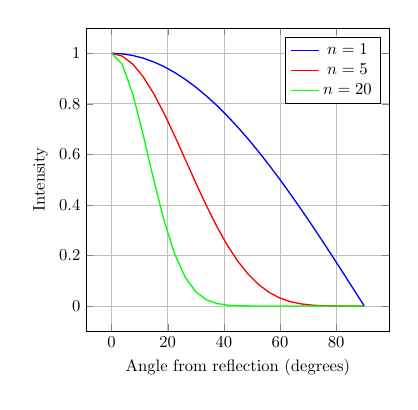
\begin{tikzpicture}[scale=0.6]
        % Plot of cosine functions with different powers
        \begin{axis}[
            width=8cm,
            height=8cm,
            domain=0:90,
            xlabel={Angle from reflection (degrees)},
            ylabel={Intensity},
            legend pos=north east,
            grid=major
          ]
          \addplot[blue, thick] {(cos(x))^1};
          \addlegendentry{$n=1$}
          \addplot[red, thick] {(cos(x))^5};
          \addlegendentry{$n=5$}
          \addplot[green, thick] {(cos(x))^20};
          \addlegendentry{$n=20$}
        \end{axis}
      \end{tikzpicture}
    \end{column}
  \end{columns}
\end{frame}

\begin{frame}{Complete Phong Equation Assembly}
  \begin{mathbox}{Putting It All Together}
    \textbf{Complete Phong illumination model:}
    \begin{align*}
      I &= I_{\text{ambient}} + I_{\text{diffuse}} + I_{\text{specular}}
    \end{align*}

    \pause
    \begin{align*}
      \mathbf{I} &= \mathbf{k}_a \odot \mathbf{I_a} + \sum_{i=1}^{n} \mathbf{I_{l_i}} \odot \left[ \mathbf{k}_d \max(0, \mathbf{N} \cdot \mathbf{L}_i) + \mathbf{k}_s \max(0, \mathbf{R}_i \cdot \mathbf{V})^n \right]
    \end{align*}
  \end{mathbox}
\end{frame}

\subsection{Blinn-Phong Model}

\begin{frame}{Blinn-Phong: A More Efficient Alternative}
  \begin{columns}
    \begin{column}{0.6\textwidth}
      \begin{raybox}{Motivation for Blinn-Phong}
        \footnotesize
        \textbf{Problem with Phong:} Computing the reflection vector $\mathbf{R}$ is expensive
        \begin{align*}
          \mathbf{R} = 2(\mathbf{N} \cdot \mathbf{L})\mathbf{N} - \mathbf{L}
        \end{align*}

        \vspace{0.3cm}
        \pause
        \textbf{Jim Blinn's solution (1977):} Use a halfway vector instead

        \vspace{0.3cm}
        \pause
        \textbf{Key insight:}
        \begin{itemize}
          \item When $\mathbf{V} = \mathbf{R}$, the halfway vector $\mathbf{H}$ equals the normal $\mathbf{N}$
          \item We can measure the angle between $\mathbf{H}$ and $\mathbf{N}$ instead
          \item Much cheaper to compute!
        \end{itemize}
      \end{raybox}
    \end{column}
    \begin{column}{0.4\textwidth}
      \begin{tikzpicture}[scale=0.8]
        % Surface
        \draw[ObjectColor, very thick] (-2,0) -- (2,0);
        \fill[ObjectColor] (0,0) circle (3pt);
        \draw[->, PrimaryColor, thick] (0,0) -- (0,1.5) node[above,black] {\footnotesize $\mathbf{N}$};
        \draw[->, lightray, thick] (0,0) -- (135:1.5) node[left,black] {\footnotesize $\mathbf{L}$};

        \draw[->, AccentColor, thick] (0,0) -- (15:1.5) node[right] {\footnotesize $\mathbf{V}$};

        \draw[->, PrimaryColor, thick] (0,0) -- (45:1.5) node[right] {\footnotesize $\mathbf{R}$};

        \only<2->{
          \draw[->, red, very thick] (0,0) -- (75:1.5) node[right] {\footnotesize $\mathbf{H}$};

          \node[below] at (0,-0.5) {\footnotesize Halfway vector bisects};
          \node[below] at (0,-0.8) {\footnotesize $\mathbf{L}$ and $\mathbf{V}$};

          \draw[-] (0, 1) arc [start angle=90, end angle=75, radius=1cm];
        }
      \end{tikzpicture}
    \end{column}
  \end{columns}
\end{frame}

\begin{frame}{Blinn-Phong Mathematics and Comparison}
  \begin{columns}
    \begin{column}{0.5\textwidth}
      \begin{mathbox}{Blinn-Phong Formula}
        \footnotesize
        \textbf{Halfway vector calculation:}
        \begin{align}
          \mathbf{H} = \frac{\mathbf{L} + \mathbf{V}}{|\mathbf{L} + \mathbf{V}|}
        \end{align}

        \textbf{Specular term:}
        \begin{align}
          I_{\text{spec}} = \mathbf{k}_s \odot \mathbf{I}_l \max(0, \mathbf{N} \cdot \mathbf{H})^{n'}
        \end{align}

        where $n'$ is typically 2-4 times larger than Phong's $n$

        \vspace{0.3cm}
        \pause
        \textbf{Performance comparison:}
        \begin{itemize}
          \item \textbf{Phong:} 5 operations (2 dot products, 1 scalar multiply, 2 vector ops)
          \item \textbf{Blinn-Phong:} 4 operations (1 vector add, 1 normalize, 1 dot product)
        \end{itemize}
      \end{mathbox}
    \end{column}
    \begin{column}{0.5\textwidth}
      \begin{figure}
        \centering
        \includegraphics[width=0.9\linewidth]{images/blinn-phong.png}
        \caption*{\scriptsize Blinn-Phong vs Phong}
      \end{figure}
    \end{column}
  \end{columns}
\end{frame}